% !TeX program = lualatex
\documentclass[tikz,border=2pt]{standalone}

\usepackage{pgfplots}
\pgfplotsset{compat=1.18}
\usetikzlibrary{shapes.geometric}
\usepgfplotslibrary{fillbetween}
\usepackage[colorlinks=true,linkcolor=blue,urlcolor=blue]{hyperref}


\usetikzlibrary{patterns,decorations.markings}
\tikzset{
photon/.style={
decorate,
decoration={snake, amplitude=1.5pt, segment length=3pt},
thick
},
}

\begin{document}

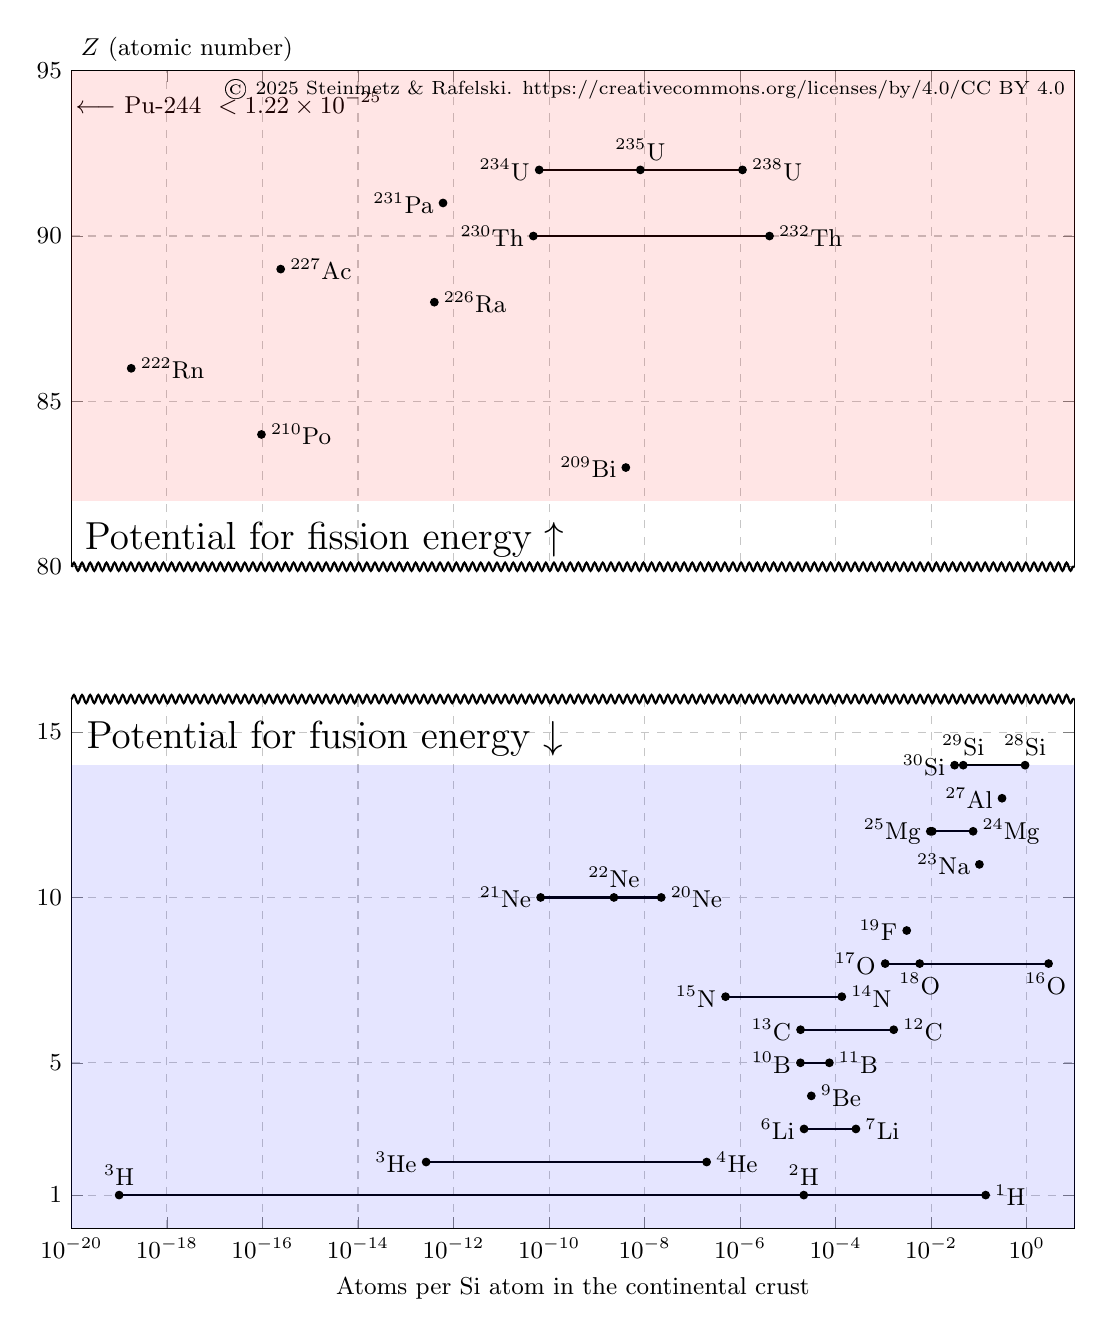
\begin{tikzpicture}[scale=0.98, transform shape]
\begin{axis}[
width=13.0cm, height=15.0cm,
xlabel={Atoms per Si atom in the continental crust},
ylabel={$Z$ (atomic number)},
xmode=log,
log basis x=10,
xmin=1e-20, xmax=1e1,
ymin=0, ymax=35, % compressed axis: 0--15, gap, then 80--95 mapped to 20--35
xmajorgrids,
xminorgrids,
ymajorgrids,
major grid style={dashed, gray!45},
minor grid style={dashed, gray!25},
ytick={1,5,10,15,20,25,30,35},
yticklabels={1,5,10,15,80,85,90,95},
tick label style={font=\small},
label style={font=\small},
clip=false,
only marks,
mark=*,
scale only axis,
ylabel style={
  rotate=-90,
  at={(axis description cs:0,1.0)},
  anchor=south west,
  yshift=0pt,
},
]

\addplot[
only marks,
mark=*,
mark size=1.4pt,
nodes near coords={{\pgfplotspointmeta}},
point meta=explicit symbolic,
% Bind table columns to macros for this point:
visualization depends on={value \thisrow{anc}  \as \ANC},
visualization depends on={value \thisrow{yoff} \as \YOFF},
visualization depends on={value \thisrow{xoff} \as \XOFF},
% Use them for the label position:
every node near coord/.style={
  font=\small,
  anchor=\ANC,
  yshift=\YOFF,
  xshift=\XOFF,
},
] table[row sep=\\, meta=label, x=ratio, y=Z] {
Z  ratio         label           anc    yoff  xoff \\
1  0.137978508   $^{1}$H          west   0pt   0pt \\
1  2.15E-05      $^{2}$H          south  0pt   0pt \\
1  1.00E-19      $^{3}$H          south  0pt   0pt \\
2  2.67E-13      $^{3}$He         east   0pt   0pt \\
2  1.99E-07      $^{4}$He         west   0pt   0pt \\
3  2.18E-05      $^{6}$Li         east   0pt   0pt \\
3  0.00026522    $^{7}$Li         west   0pt   0pt \\
4  3.09E-05      $^{9}$Be         west   0pt   0pt \\
5  1.83E-05      $^{10}$B         east   0pt   0pt \\
5  7.38E-05      $^{11}$B         west   0pt   0pt \\
6  0.001641611   $^{12}$C         west   0pt   0pt \\
6  1.84E-05      $^{13}$C         east   0pt   0pt \\
7  0.000134505   $^{14}$N         west   0pt   0pt \\
7  4.95E-07      $^{15}$N         east   0pt   0pt \\
8  2.863171122   $^{16}$O         north  0pt  -1pt \\
8  0.00108773    $^{17}$O         east   0pt   0pt \\
8  5.74e-03      $^{18}$O         north  0pt   0pt \\
9  0.00307       $^{19}$F         east   0pt   0pt \\
10 2.23E-08      $^{20}$Ne        west   0pt   0pt \\
10 6.66E-11      $^{21}$Ne        east   0pt   0pt \\
10 2.28e-09      $^{22}$Ne        south  0pt   0pt \\
11 0.102         $^{23}$Na        east   0pt   0pt \\
12 0.075398205   $^{24}$Mg        west   0pt   0pt \\
12 0.0095691     $^{25}$Mg        east   0pt   0pt \\
13 0.304         $^{27}$Al        east   0pt   0pt \\
14 0.9222968     $^{28}$Si        south  0pt   0pt \\
14 4.68e-02      $^{29}$Si        south  0pt   0pt \\
14 0.0308716     $^{30}$Si        east   0pt   0pt \\
% --- heavy region mapped: Z' = Z - 60 ---
%22 9.42E-08      $^{204}$Pb      east   0pt   0pt \\ % 82 - 60
%22 3.53E-06      $^{208}$Pb      west   0pt   0pt \\
%22 1.62E-06      $^{206}$Pb      south  0pt  -15pt \\
%22 1.49E-06      $^{207}$Pb      south  0pt   14pt \\
23 4.05E-09      $^{209}$Bi       east   0pt   0pt \\ % 83 - 60
24 9.53E-17      $^{210}$Po       west   0pt   0pt \\ % 84 - 60
26 1.79E-19      $^{222}$Rn       west   0pt   0pt \\ % 86 - 60
28 3.97E-13      $^{226}$Ra       west   0pt   0pt \\ % 88 - 60
29 2.41E-16      $^{227}$Ac       west   0pt   0pt \\ % 89 - 60
30 4.12E-06      $^{232}$Th       west   0pt   0pt \\ % 90 - 60
30 4.69E-11      $^{230}$Th       east   0pt   0pt \\
31 6.03E-13      $^{231}$Pa       east   0pt   0pt \\ % 91 - 60
32 6.22E-11      $^{234}$U        east   0pt   0pt \\ % 92 - 60
32 1.12E-06      $^{238}$U        west   0pt   0pt \\
32 8.14E-09      $^{235}$U        south  0pt   0pt \\
% Additional isotopes without labels (names in comments)
12 1.05e-02      {}               west   0pt   0pt \\ % Mg-26
};


% Pu-244 (theoretical) label (94 -> 34)
\node[font=\small, anchor=west, xshift=-2pt]
at (axis cs:1e-20,34) {$\longleftarrow$ Pu-244 \ $<1.22\times10^{-25}$};

% Hydrogen isotopes: from t (1e-19) to d (2.15e-05) to p (1.38e-01) at Z=1
%\draw[black, thick] (axis cs:2.15e-05,1) -- (axis cs:1.38e-01,1);
\draw[black, thick] (axis cs:1e-19,1) -- (axis cs:1.38e-01,1);

% Helium isotopes: from He-3 (2.67e-13) to He-4 (1.99e-07) at Z=2
\draw[black, thick] (axis cs:2.67e-13,2) -- (axis cs:1.99e-07,2);

% --- Isotope-span lines (horizontal: min ↔ max at fixed Z) ---
% light region up to Si
\draw[black, thick] (axis cs:2.18e-05,3) -- (axis cs:0.00026522,3);
\draw[black, thick] (axis cs:1.83e-05,5) -- (axis cs:7.38e-05,5);
\draw[black, thick] (axis cs:1.84e-05,6) -- (axis cs:0.001641611,6);
\draw[black, thick] (axis cs:4.95e-07,7) -- (axis cs:0.000134505,7);
\draw[black, thick] (axis cs:0.00108773,8) -- (axis cs:2.863171122,8);
\draw[black, thick] (axis cs:6.66e-11,10) -- (axis cs:2.23e-08,10);
\draw[black, thick] (axis cs:0.0095691,12) -- (axis cs:0.075398205,12);
\draw[black, thick] (axis cs:0.0308716,14) -- (axis cs:0.9222968,14);
% heavy region (Pb and actinides mapped)
%\draw[black, thick] (axis cs:9.42e-08,22) -- (axis cs:3.53e-06,22); % Pb
\draw[black, thick] (axis cs:4.69e-11,30) -- (axis cs:4.12e-06,30); % Th
\draw[black, thick] (axis cs:6.22e-11,32) -- (axis cs:1.12e-06,32); % U

\path[fill=white,  fill opacity=1.0]
(axis cs:9e-21,16) rectangle (axis cs:1.1e1,20);
\draw[photon] (axis cs:1e-20,16) -- (axis cs:1e1,16);
\draw[photon] (axis cs:1e-20,20) -- (axis cs:1e1,20);

% --- background spans ---
\path[fill=blue, fill opacity=0.10]
(axis cs:1e-20,0) rectangle (axis cs:1e1,14);

\path[fill=red,  fill opacity=0.10]
(axis cs:1e-20,22) rectangle (axis cs:1e1,35); % mapped 82--95 -> 22--35

% Fission/Fusion Boundary
\node[font=\Large, anchor=south, yshift=0pt] at (axis cs:2e-15,20) {Potential for fission energy $\uparrow$};

\node[font=\Large, anchor=south, yshift=0pt] at (axis cs:2e-15,14) {Potential for fusion energy $\downarrow$};

% Copyright notice
\node[font=\scriptsize, anchor=north east, yshift=0pt]
at (axis description cs:1.0,1.0) {\textcopyright\ 2025 Steinmetz \& Rafelski. \href{https://creativecommons.org/licenses/by/4.0/}{CC~BY~4.0}};

\end{axis}
\end{tikzpicture}

\end{document}